\documentclass{article}
\usepackage[T1]{fontenc}
\usepackage{geometry}
\geometry{a4paper, left=20mm, right=20mm, top=20mm, bottom=20mm}
\usepackage[margin=1.2in]{geometry}
\usepackage{graphicx}
\usepackage{listings}
\begin{document}

\title{Assignment Report - Monte Carlo Simulation}
\author{Gokul K\\[2\baselineskip]
Roll Number: 21\\[2\baselineskip]}
\date{\today}

\maketitle

\large
\section{Problem Statement}
Use Monte Carlo simulation to find the average height

\section{Theory}
Monte Carlo simulation is a computerized mathematical technique
used for risk analysis in a large number of fields such as finance,
project management, energy, manufacturing, engineering etc. In Monte  
Carlo simulations instead of solving a complex or an impossible problem,
we run a large number of simulations using random numbers that falls in
the range of the mathematical problem we are trying to solve.

For estimating the average height of a population, it is impractical
to collect and take arithmetic mean of the whole population. So in 
Monte Carlo simulation of the above problem we select a large optimal number 
of people randomly and ask their height and find its average. We can safely 
assume this to be closer to the mean height of the entire population

Let us assume we have an exhaustive dataset of heights of people in the population 
we are interested in.It might be practically impossible or infeasible to calculate 
the mean or expected value of height using conventional methods since the number of 
records in the dataset may be too high. So instead we run a Monte Carlo simulation 
with a large but  feasible number of trials. In each trail we pick a random record from 
the dataset and average all those randomly picked data to find an estimate of the 
actual average.

\section{Algorithm}
\begin{enumerate}
    \item Load a dataset with large number of height values
    \item Repeat 1000 times
    \begin{enumerate}
        \item Generate a random number between 0 and size of the dataset
        \item Find the height at that position in dataset
        \item Add it to a variable called sum (with initial value 0)
    \end{enumerate}
    \item Find average by dividing sum with 1000
\end{enumerate}

\section{Source Code}
\small
\begin{lstlisting}[language=Python]
import math
import random
import pandas


class MonteCarloSimulation:
    def __init__(self, no_of_samples: int, no_of_tries: int):
        self.no_of_samples = no_of_samples
        self.no_of_tries = no_of_tries
    
    def read_dataset(self, file_path: str, col_name: str):
        self.data_frame = pandas.read_csv(file_path)[col_name]
    
    def start(self):
        self.predicted_avg: float = 0
        sum: float = 0
        
        for i in range(self.no_of_tries):
            random_index = math.floor(self.no_of_samples * random.random())
            sum += self.data_frame[random_index]
        
        self.predicted_avg = sum / self.no_of_tries
        print(f"Predicted average: {self.predicted_avg}")
    
    def calculate_accuracy(self):
        real_avg: float = sum(self.data_frame) / self.no_of_samples
        print(f"Real average: {real_avg}")
        print(f"Accuracy: {100 - abs(real_avg-self.predicted_avg)/real_avg}")


    

if __name__ == '__main__':
    simulation: MonteCarloSimulation = MonteCarloSimulation(10000, 1000)
    simulation.read_dataset("height.csv", "Height")
    simulation.start()
    simulation.calculate_accuracy()
\end{lstlisting}

\section{Output}
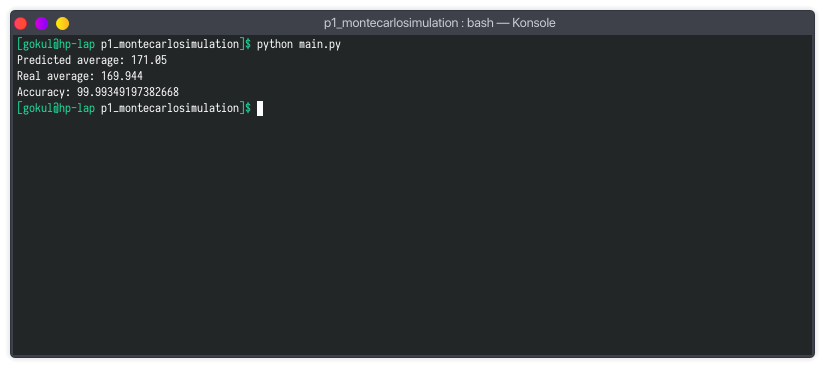
\includegraphics[width=\textwidth]{img/ss.png}
\section{Result}
\large
We were able to calculate an approximate value for the average height
through Monte Carlo Simulation with only one-tenth of the calculations 
required to compute the real average.
\end{document}